\chapter{Introduction}

\section{Zero Point Energy and the Dynamical Casimir Effect}\label{sec:ZPE_and_DCE}

One of the most exciting predictions of quantum field theory is the existence of quantum vacuum fluctuations. Fluctuations in the fields permeating the vacuum have lead us to re-think the nature of "empty" space. Quantum theory predicts the existence of a vacuum state, where no particles are present, yet with a non-zero energy. The existence of this zero-point energy in the quantum electromagnetic field has observable implications in different physical phenomena. Some of phenomena in the field of quantum electrodynamics (QED) which are consequences of the zero-point energy include the Lamb shift \cite{Lamb1947}, where the interaction of electrons with the underlying vacuum leads to a detectable energy difference between energy states in hydrogen atoms, as well as the (static) Casimir effect \cite{Casimir1948}, where two conducting plates experience a force between them explained by the difference between the vacuum energy between the plates and on the space surrounding them. 

Of particular interest to us is a phenomenon where the effects of the zero-point energy can be observed in the presence of the time-dependent modulation of a boundary. First proposed half a century ago by Moore \cite{Moore1970}, the dynamical Casimir effect (DCE) refers to the spontaneous creation of photons by the excitation of the zero-point quantum states due to a moving mirror (see Fig.\,\ref{fig:Nation_movingmiror}). Moore showed that the effect was "immeasurably small" for non-relativistic mirror trajectories. Therefore, the detection of DCE would only be possible in scenarios with boundaries exhibiting relativistic motion.
%
\begin{figure}
    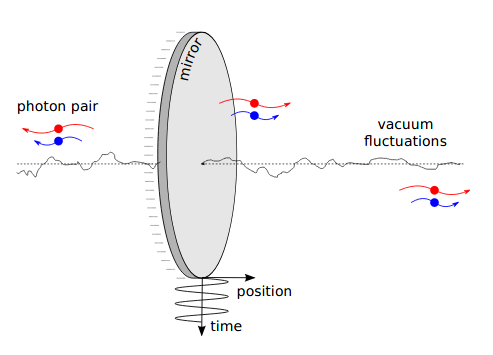
\includegraphics[width = 3.7in, keepaspectratio]{figures/intro/Nation2011_DCE.png}
    \caption{Illustration of the dynamical Casimir effect (DCE) due to an oscillating mirror. 
    Photon pairs are created out of vacuum fluctuations by means of the non-adiabatic oscillation of a mirror. Credit: \protect\cite{Nation2011}.}
    \label{fig:Nation_movingmiror}
\end{figure}
\newpage
\noindent
For a perfect mirror (no transmission), undergoing an oscillatory motion with frequency $\Omega$, and oscillation amplitude $a$, 
the number of photon pairs produced per unit time is
%
\begin{equation}
    \frac{N}{T} = \frac{\Omega}{3\pi}\left(\frac{v}{c}\right)^2 
\end{equation}
%
where $v = \Omega \, a$ is the maximum speed of the mirror \cite{Lambrecht1996}. Thus, to produce a significant amount of photons requires
a mirror which oscillates at speeds close to the speed of light.

Since the original proposal by Moore, the study of the DCE has evolved into a mature field with many publications analyzing theoretical implications as well as experimental realizations (see \cite{Dodonov_Review2020}). Different treatments of the DCE can be found in the literature, where states of the quantum electromagnetic field are characterized by its energy momentum tensor $T_{\alpha, \beta}(x,t)$ \cite{Fulling&Davies1976}, or by means of a second-quantization expansion of the fields in the Fock state basis \cite{Dodonov1990}. In this work, we employ the latter approach as it allows us to examine the field in terms of its photon statistics similar to the ones employed in \cite{Dodonov1990,Lambrecht1996, Nation2011}.

\begin{figure}
    %
    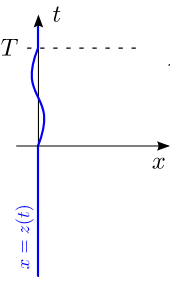
\includegraphics[width=1.3in, keepaspectratio]{figures/intro/Nation2011_transformation.png}
    \caption{Oscillation of a mirror as a function of time. Using a Bogoliubov transformation we express the field modes 
    at times $t>T$ as a superposition of field modes for $t<0$. Credit: \protect\cite{Nation2011}.}
    \label{fig:Nation_transformation}
\end{figure}

\newpage

Consider a scattering-type problem of a field $\phi(x,t)$ in 1+1 dimensional space-time. 
The field has a boundary condition which undergoes some time-dependent 
change in positions between times $t=0$ and $t=T$ (see Fig.\,\ref{fig:Nation_transformation}). We can write our field as an expansion 
of modes at the stationary regions $t<0$ and $t>T$ respectively:
%
\begin{gather}
    \phi_{\,\text{in}}(x,t) = \sum_n \left[ \psi_n^{(0)}(x,t) \, a_n + \text{h.c.}\right] \, \, ,\label{eq:fields_bogoliubov1}
    \\
    \phi_{\,\text{out}}(x,t) = \sum_n \left[ \psi_n(x,t) \, b_n + \text{h.c.}\right] \, \, .\label{eq:fields_bogoliubov2}
\end{gather}
%
Here we have assumed that the field has a discrete set of basis states. In general, the sums in 
Eqs.\,(\ref{eq:fields_bogoliubov1}), (\ref{eq:fields_bogoliubov2}) will be replaced by an integral over a continuous set of basis states. 
The modes of the field for $t>T$ are not the same as for $t<0$, but they can be expressed as a linear superposition of these 
modes by means of a Bogoliubov transformation:
%
\begin{equation}\label{eq:bogoliubov_trans}
    \begin{split}
    b_m = \sum_n \left(\alpha_{nm} \, a_n \, + \, \beta_{nm} \, a_n^{\dagger} \right) \, \, ,
    \\
    b_m^{\dagger} = \sum_k \left(\alpha_{nm}^* \, a_n^{\dagger} \, + \, \beta_{nm}^* \, a_n \right) \, \, ,
    \end{split}
\end{equation}
%
with the normalization $\sum_n \left(|\alpha_{nm}|^2 + |\beta_{nm}|^2\right) = 1$ to preserve unitarity.
Note that this transformation preserves the momentum of the field. If one interprets the operator $b_m$ as annihilating a photon 
with momentum $k$, then one can interpret the r.h.s.\,of the first line 
of Eq.\,(\ref{eq:bogoliubov_trans}) as a term that annihilates a photon 
with momentum $k$, ($a_n$), plus another term that creates a particle with momentum $-k$, ($a_n^{\dagger}$). Thus the momentum 
of the field in conserved. A similar conclusion applies to the creation operator $b_m^{\dagger}$.
Thus, photon statistics for both regions in Eqs.\,(\ref{eq:fields_bogoliubov1}), (\ref{eq:fields_bogoliubov2}) are well-defined.

We can thus find the final number of photons. For an initial field in the vacuum state ($\lvert0\rangle$), 
%
\begin{equation}\label{eq:bogoliubov_dce}
\begin{aligned}
    N^{\text{out}}_m &= \left\langle b_m^{\dagger} \, b_m \right\rangle_{\text{in}}\\
    %
    &= \sum_n
    \left\langle
    \left(
    |\alpha_{nm}|^2 \, a_n^{\dagger} \, a_n \, + \, 
    |\beta_{nm}|^2 \, a_n \, a_n^{\dagger}
    \right)
    \right\rangle_{\text{in}}\\
    %
    &= \sum_n
    \left\langle
    \left(
    a_n^{\dagger} \, a_n \, + \, |\beta_{nm}|^2 
    \right)
    \right\rangle_{\text{in}}\\
    %
    &= \sum_n |\beta_{nm}|^2 \, \, .
\end{aligned}
\end{equation}
%
This shows a non-zero number of photons in the final state of the field, even though we started from the vacuum state, as long as there are coefficients $\beta_{nm} \neq 0$. The mixing of terms due to the scattering with a time-dependent boundary expressed through the Bogoliubov transformation 
in Eq.\,(\ref{eq:bogoliubov_trans}), combined with the commutation relations of the creation/annihilation operators ($a_n^{\dagger}, a_n $), 
gives rise to the creation of DCE photons. The problem of calculating the number of DCE photons generated when there is a time-dependent modulation of the boundary condition is then equivalent to that of finding these Bogoliubov coefficients, given an initial set of basis states for the static fields. 

%---------------------------------------------------------------------------------------------

\section{Superconducting quantum circuits and SQUIDs}\label{sec:SC_and_SQUIDs}

The quantum electromagnetic field is largely studied via the interactions between light and matter, by placing atoms in low loss optical cavities where they interact with a quantized electromagnetic field. This is the field of cavity QED, where experiments are done with light in the optical domain. An alternative regime is that of superconducting quantum circuits (SQC), which usually operate in the microwave regime. In this field, the role of atoms in cavity QED is taken by superconducting artificial atoms, which are quantum multi-level systems created using Josephson junctions and superconducting circuit elements \cite{Gu2017}. Josephson junctions are created by interrupting two superconductor segments by a insulating (non-superconducting) gap (see Fig.\,\ref{fig:Kittel_JJ}). The Josephson effect, which describes Cooper pairs tunneling across this insulating gap, gives SQC non-linearity without introducing dissipation.
Advances in the theory and technology of superconducting circuits have developed rapidly due to their use in quantum computing and other quantum technologies \cite{Krantz2019}.
Treatments for the quantum description of SQC, including the quantization method, and the input-output formalism we employ can be found in standard references for quantum network theory \cite{Yurke1984, Vool2017}.

\begin{figure}[ht]
    %
    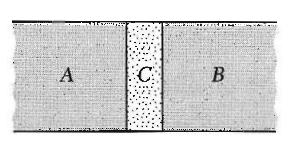
\includegraphics[width=2in, keepaspectratio]{figures/intro/Kittel_Josephson.png}
    \caption{Schematic representation of a Josephson junction. Superconducting segments A and B are interrupted by a thin insulating barrier C. Credit: \protect\cite{Kittel1996_Solid_State}.}
    \label{fig:Kittel_JJ}
\end{figure}

\begin{figure}
    %
    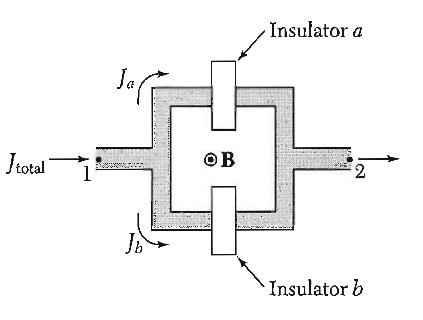
\includegraphics[width=2in, keepaspectratio]{figures/intro/Kittel_SQUID.png}
    \caption{Schematic representation of a superconducting quantum interference device (SQUID). A superconducting loop is interrupted by two Josephson junctions with total current $J_{\text{total}}$. An external magnetic field $B$ is applied to the loop. Credit: \protect\cite{Kittel1996_Solid_State}.}
    \label{fig:Kittel_SQUID}
\end{figure}

There are two elements of a such circuits relevant for our work. The first one is the superconducting transmission line, realized through coplanar waveguides (CPW) which consist of a central conductor surrounded by a ground plane. The second one is the superconducting quantum interference device (SQUID), which consists of a superconducting loop interrupted by two Josephson junctions.
Treatments for the quantum description of SQC, including the quantization method, and the input-output formalism 
we employ in our quantum network theory treatment can be found in \cite{Yurke1984, Vool2017}. 
The CPW can be modeled as a series of coupled inductor-capacitor (LC) circuits. 

\begin{figure}[ht]
    %
    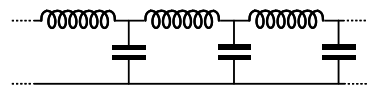
\includegraphics[width=0.5\textwidth,keepaspectratio]{figures/intro/LC_Vool2017.png}
    \caption{A superconducting coplanar waveguide (CPW) modeled as a series of inductors and capacitors. Credit: \protect\cite{Vool2017}.}
    \label{fig:CPW_diagram}
\end{figure}

We describe the dynamics by introducing the magnetic flux $\Phi_i$ at site $i$. The Lagrangian density for the flux in the CPW is then
%
\begin{equation}\label{eq:CPW_lagrangian}
\mathcal{L} = \, \frac{1}{2} \sum_i \left( \Delta x \, C_{0} \left(\dot{\Phi}_{i}\right)^{2} \, - \, 
\frac{\left(\Phi_{i+1}-\Phi_{i}\right)^{2}}{\Delta x \, L_{0}} \right)
\end{equation}
%
where $\Delta x$ is the distance between nodes and $C_0$, $L_0$ are the capacitance and inductance per unit length, respectively. This Lagrangian has a similar form to the one for a mechanical oscillator. The node fluxes take the place of position coordinates, while node charges take the place of momentum. The capacitive term in the Lagrangian takes the role of kinetic energy, while the inductive term takes the role of potential energy.
As for the SQUID, it also contains capacitive and inductive terms. The total inductive energy of the SQUID is
%
\begin{equation}\label{eq:squid_energy_assym}
    E_{\text{SQUID}}(t) = - E_{J_1} \cos{\left(2\pi
    \frac{\Phi_{J_1}}{\Phi_0}\right)} - E_{J_2} \cos{\left(2\pi
    \frac{\Phi_{J_2}}{\Phi_0}\right)} \, \, ,
\end{equation}
%
where $E_{J_\alpha}$ and $\Phi_{J_\alpha}$ are the Josephson energy and the flux through the $\alpha$th Josephson junction, 
respectively, $\Phi_0$ is the magnetic flux quantum, and the fluxes of Josephson junctions are related to the external flux
by $\Phi_1 - \Phi_2  = \Phi_{\text{ext}}(t)$. If we consider a symmetric SQUID, such that $E_{J_1} = E_{J_2} = \epsilon_J$ and
$C_{J_1} = C_{J_2} = C_J/2$, we can write the Lagrangian density for the SQUID as
%
\begin{equation}\label{eq:squid_energy_symm}
    E_{\text{SQUID}}(t) = -2E_J \left|\cos\left(\pi\frac{\Phi_{\text{ext}}(t)}{\Phi_0}\right)\right|
    \cos\left(2\pi \frac{\Phi_J}{\Phi_0} \right) \, \, .
\end{equation}
%
One may think of the SQUID as a single Josephson junction with a tunable inductance which depends on the applied magnetic flux. For a regular inductor, the energy is stored in the magnetic field passing through the coil of the inductor. For a Josephson junction, the inductance is related to the kinetic energy of Cooper pairs through the junction.

%---------------------------------------------------------------------------------------------

\section{DCE in Superconducting Circuits}\label{sec:DCE_in_SC}

The superconducting microwave circuit regime has proved a promising platform to study vacuum energy amplification phenomena \cite{Nation2011} such as the Unruh effect, parametric amplification, and an analogue Hawking radiation. More importantly for our work, this regime is where the first experimental evidence of DCE has been achieved \cite{Wilson2011_ObservationDCE}. 

In work by Johansson et al.\,\cite{Johansson2009, Johansson2010}, an architecture consisting of a semi-infinite CPW terminated by a SQUID is proposed. By applying an external magnetic flux across the SQUID, the authors show that the boundary condition imposed by the SQUID mimics that of a perfectly reflecting mirror at an effective distance $L^0_{\text{eff}}$ from the SQUID (see Fig.\,\ref{fig:Johansson2010_effectivemirror}). This distance is given by
%
\begin{equation}\label{eq:squid_inductance}
    L^0_{\text{eff}} = \frac{L_J(\Phi_{\text{ext}})}{L_0} \, \, ,
\end{equation}
%
where $L_J(\Phi_{\text{ext}})$ is the Josephson inductance of the SQUID and $L_0$ is the inductance per unit length of the CPW. Applying a harmonic modulation of the external magnetic flux it is thus possible to reproduce the boundary condition of an oscillating mirror, resulting in DCE radiation. The influence of the external flux on the SQUID inductance is large enough so that a small modulation in the flux is equivalent to a significant effective amplitude of oscillation for a mirror 
(see Fig.\,\ref{fig:Johansson2010_effectivemirror}). 
The bias lines adjacent to SQUIDs can implement frequencies of oscillation in the range of tens of GHz. The combination of "large" amplitudes and frequencies of oscillation make a SQUID a suitable candidate for detecting DCE radiation (see Section \ref{sec:ZPE_and_DCE}). 
Figure \ref{fig:Johansson2010_reproduced} shows results reproduced by our calculations using the analysis in \cite{Johansson2010}. 
The photon number density is shown as a function of frequency.
%
\begin{figure}
    %
    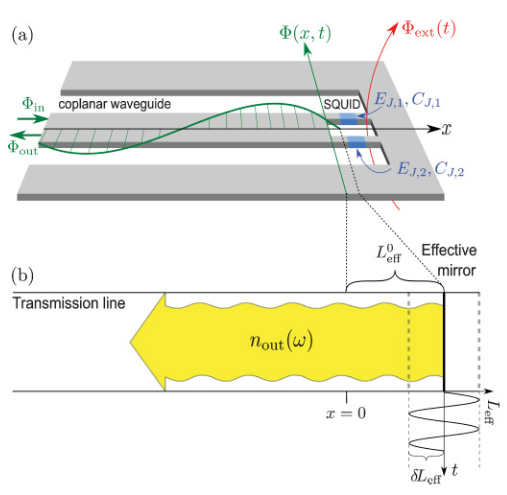
\includegraphics[width=3in, keepaspectratio]{figures/intro/Johansson2010_effectivemirror.png}
    \caption{(a) Representation of a coplanar waveguide (CPW) terminated by a superconducting quantum interference device (SQUID). 
    The external harmonic magnetic flux $\Phi_{\text{ext}}(t)$ generates 
    the boundary condition of an oscillating mirror (b) located at an effective distance $L^0_{\text{eff}}$ from the SQUID at $x=0$. The mirror oscillates with amplitude $\delta L_{\text{eff}}$. The oscillation mirror produces DCE radiation. Credit: \protect\cite{Johansson2010}.}
    \label{fig:Johansson2010_effectivemirror}
\end{figure}


\begin{figure}
    %
    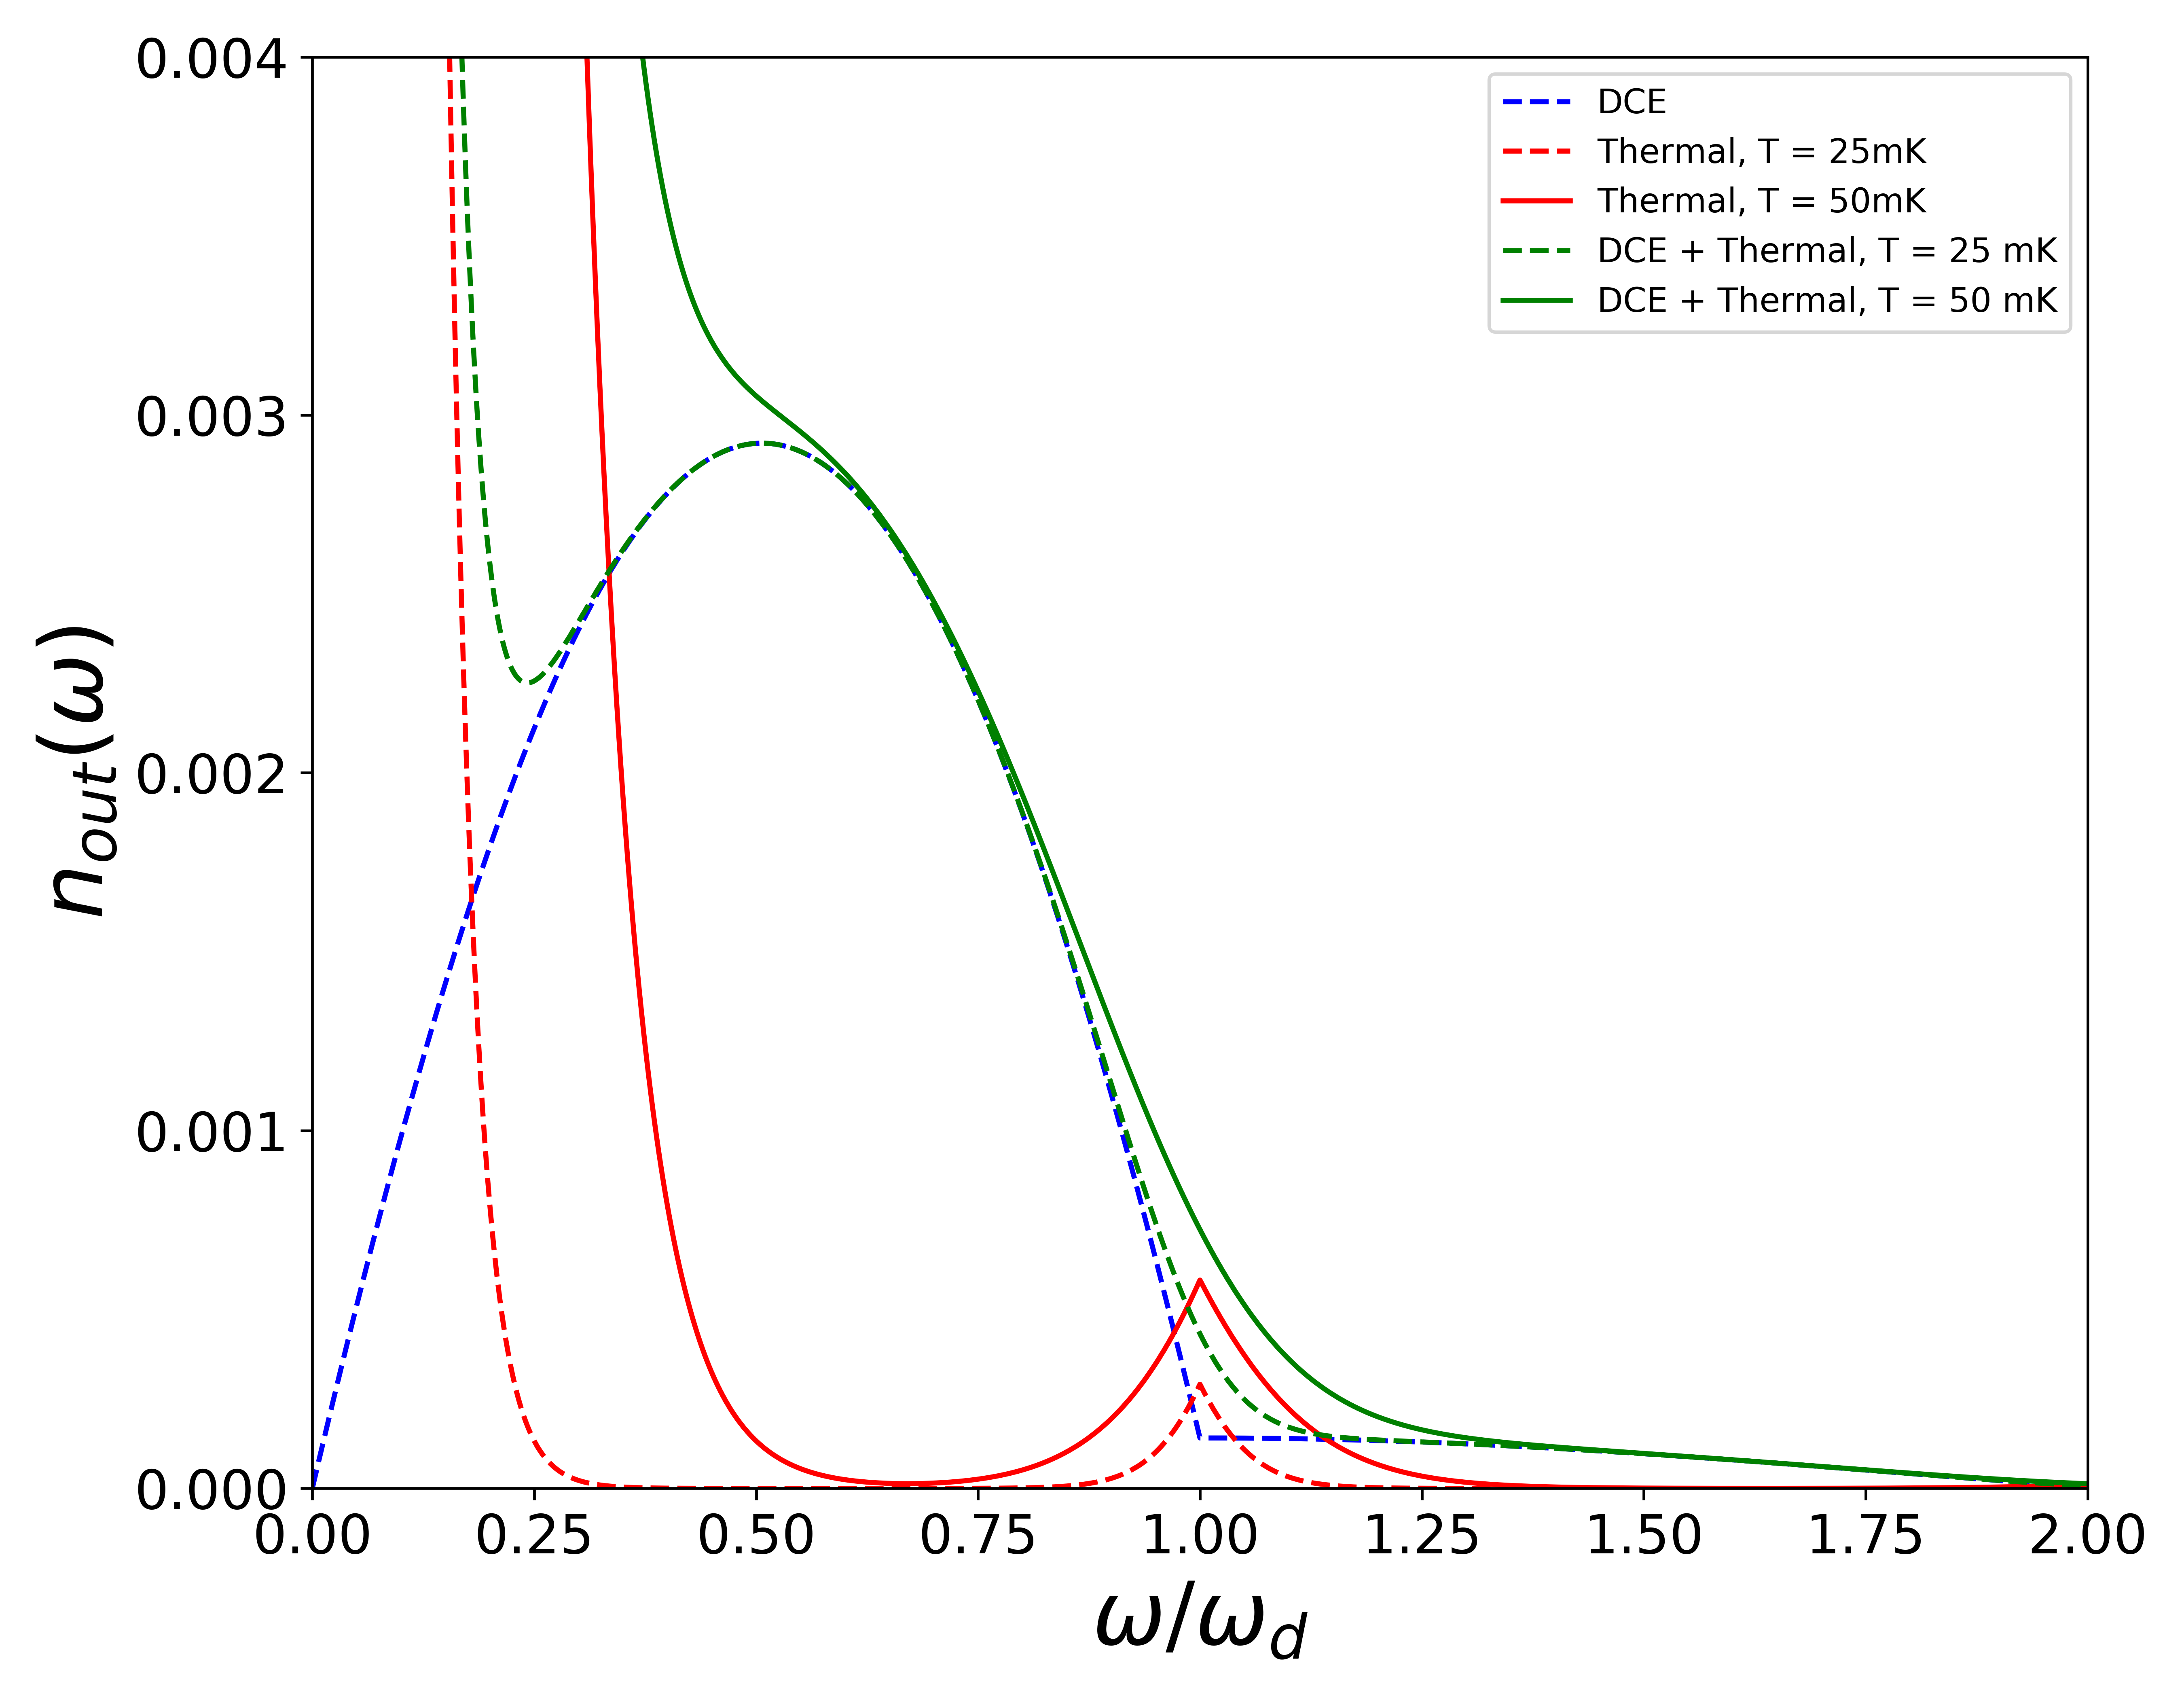
\includegraphics[width=6.5in,keepaspectratio]{figures/intro/reproduced_Johansson.png}
    \caption{Reproduced results using the analysis from \protect\cite{Johansson2010}. 
    Shown is the photon number as a function of frequency in units of the SQUID driving frequency $\omega_d / 2\pi$ = 18.6GHz. The output thermal radiation is shown for temperatures of 25mK and 50mK and compared with the DCE radiation emitted.}
    \label{fig:Johansson2010_reproduced}
\end{figure}

\newpage
The DCE was observed experimentally in work by Wilson et. al. \cite{Wilson2011_ObservationDCE}. The radiation emitted showed two-mode squeezing, which is a signature of the pair-creation quantum process in the DCE. Shortly after, other realizations for DCE in superconducting circuits were proposed, an example being \cite{Lahteenmaki_DCE2013}, where the dielectric properties of a SQUID metamaterial resonator are modulated, corresponding to a modulated cavity length and generating DCE. The entanglement nature of superconducting DCE photons has been also investigated \cite{Johansson2013}, as well as its use as in quantum information and simulation. Some examples include \cite{Felicetti2014, Peropadre2018, Agusti2019, Zhao2021}.